\chapter{Porte}

% Eu poderia descrever como eu tenho que incluir cada classe feita em ./include/system/types.h, opções de traits, etc..


Nesta seção será discutido como foi o porte de cada mediador de hardware, explicando as decisões tomadas. Antes de entrar nas especificidades de cada componente, é interessante colocar aqui alguns conceitos comuns que são usados em cada mediador.

\section{Registradores Mapeados em Memória}
A maneira usada para se comunicar, configurar e ler o estado de um dado componente de hardware é através da leitura e/ou escrita em registradores mapeados em memória. Um registrador mapeado em memória basicamente é uma região fixa da memória, onde uma escrita naquela posição indica uma escrita no registrador lá mapeado.
Exemplificando, a UART possui um registrador chamado rcvr\_timeout\_reg0, responsável por indicar quantos ciclos\footnote{Na realidade é o número de baud\_samples que se passaram.} a UART deve esperar um novo caractere chegar antes de emitir uma interrupção de \emph{timeout}. Este registrador está mapeado na posição de memória 0xE000001C para a UART0. Portanto, para configurar que o número de ciclos esperado seja de 20, basta escrever este número naquela posição. Uma maneira de fazer esta escrita, por exemplo, em C/C++, é: \verb+*((unsigned long*)0xE000001C) = 20;+.

%\section{memory map}

%\section{Boot}

\section{Traits}

Existem 4 arquivos traits.h que devem ser levados em consideração em um porte, dois deles devem ser completamente reescritos. Os arquivos \verb+./include/traits.h+ e \verb+/include/system/traits.h+ (onde `.' é a pasta raiz do código) possuem configurações gerais do EPOS, que, a princípio, devem ser independentes de arquitetura. Na prática há alguns pequenos ajustes que devem ser feitos nesses arquivos, pois é lá que se define, por exemplo, se o EPOS trabalhará em um processador \emph{multicore}, se utilizará \emph{scratchpad}, quais componentes estarão em modo de depuração e etc; entretanto isto se resume a trocar o valor de algumas variáveis de \emph{true} para \emph{false} e vice-versa.

Os outros dois arquivos são \verb+./include/mach/zynq/traits.h+ e\\ \verb+./include/arch/armv7/traits.h+. Essa divisão é necessária pois, como dito anteriormente, é possível de um mesmo processador estar em diferentes \emph{machines}, e, caso seja necessário fazer um porte para aquela plataforma, bastaria modificar os arquivos da pasta \emph{mach}, deixando os da pasta \emph{arch} praticamente intactos, o que facilita muito novos portes.

O arquivo \verb+./include/arch/armv7/traits.h+ trata das opções específicas do processador, portanto é lá que opções como \emph{endianess}, velocidade de \emph{clock}, número de \emph{cores}, tamanho da \emph{heap} e \emph{stacks}, bem como outras opções pertinentes ao mapeamento de memória e opções da MMU podem ser configuradas.

No arquivo de traits da \emph{machine}, ficam as opções de configuração de componentes como a UART, controlador de interrupções, \emph{timer}, e qualquer componente de interfaceamento externo à placa (rede, por exemplo). Componentes podem ser facilmente ativados ou desativados nestas opções.

\section{Metaprogramação estática}

A arquitetura do EPOS usa pesadamente de metaprogramação estática para, em tempo de compilação, selecionar a arquitetura, bem como cada componente que será ou não utilizado. Por exemplo, podemos definir um \verb+if+ estático para selecionar de qual classe a classe Chronometer irá derivar. Primeiramente a definição do \verb+if+:

\begin{verbatim}
template<bool condition, typename Then, typename Else> struct IF
{
    typedef Then Result;
};
\end{verbatim}

Este template, a princípio, nada mais faz do que tomar 3 parâmetros e então criar um tipo chamado \verb+Result+ igual ao segundo parâmetro, contudo, se fizermos uma especialização deste template, ele passa ser útil:

\begin{verbatim}
template<typename Then, typename Else> struct IF<false, Then, Else>
{
    typedef Else Result;
};
\end{verbatim}

Com esta especialização, toda vez que o primeiro parâmetro resolver-se como falso, \verb+Result+ será definido como o terceiro parâmetro. Temos, portanto, um \verb+if+ metaprogramado funcional, agora voltemos ao exemplo do chronometro.

Suponha que caso a arquitetura não seja multicore, e nos traits o TSC (\emph{time stamp clock}) esteja ativo, então deseja-se que Chronometer derive de TSC\_Chronometer, do contrário de Alarm\_Chronometer.

Isto pode ser feito usando nosso \verb+if+ metaprogramado da seguinte forma:

\begin{verbatim}
class Chronometer: public
IF<Traits<TSC>::enabled && !Traits<System>::multicore,
TSC_Chronometer, Alarm_Chronometer>::Result
{/*class body*/};
\end{verbatim}

Deste modo, Chronomometer derivará de \verb+IF::Result+, que será resolvido como TSC\_Chronometer ou Alarm\_Chronometer. Note que esse exemplo também mostra um uso do Traits, onde para descobrir se o TSC está ativo, bastou ler a constante \verb+Traits<TSC>::enabled+, e, para saber se o sistema é multicore, bastou ler \verb+Traits<System>::multicore+. Todo esse processamento causa zero \emph{overhead} em tempo de execução.

\section{Porte da UART}

A inicialização da UART foi feita de acordo com o sugerido pelo manual em \cite[p.~554]{ug585}. Nesta seção será comentado as decisões tomadas na configuração inicial da UART, em particular por causa dos momentos em que o manual exigia que o desenvolvedor tomasse uma decisão.

A primeira decisão que foi necessária é a de escabelecer qual será a taxa de transmissão (\emph{Baud Rate}) da UART. 

\begin{figure}[ht!]
    \centering
    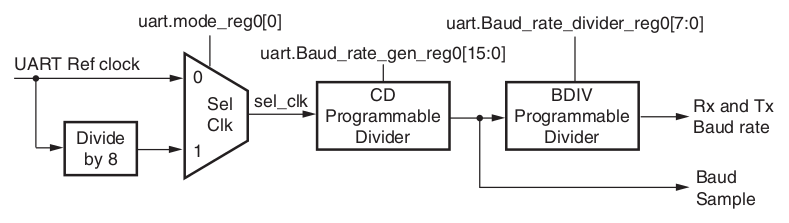
\includegraphics[width=10cm]{figuras/uart_board_rate}
    \caption{Esquemático de como é criada a taxa de transmissão.}
	\label{fig:uart}
\end{figure}

Primeiramente foi necessário configurar o \emph{clock} de referência da UART. Para isto, deve-se dividir o \emph{clock} que vem do I/O PLL (que por sua vez deriva do PS\_CLK, que é o \emph{clock} geral do sistema). Recomenda-se dividir o \emph{clock} da I/O PLL de modo a se obter 50 ou 33 MHz.
O \emph{clock} da I/O PLL, por padrão, multiplica o PS\_CLK (de 33.33 MHz) por 26, resultando num \emph{clock} de 866 MHz.
No manual diversas vezes é usado como exemplo para o \emph{clock} de referência (que é mostrado sob o nome de \verb+UART Ref clock+ na figura \ref{fig:uart}) da UART como 50 MHz, portanto, arbitrariamente, escolheu-se esse valor. Logo, deve-se configurar o registrador UART\_CLK\_CTRL, responsável por configurar o \emph{clock} de entrada da UART, para dividir este \emph{clock} vindo da I/O PLL por 17 ($866/17 = 50$).

Agora, com este \emph{clock} estabelecido, que vamos chamar de sel\_clk (de acordo com a nomenclatura do manual), devemos calcular quanto será a taxa de transmissão.
Após alguma pesquisa em fóruns de desenvolvedores de software básico, foi observado que uma taxa de transmissão de 9600 bps é bastante comum, portanto, assumindo este valor, a próxima etapa é configurar os dois divisores de \emph{clock} que ajustam a taxa de transmissão, como indicado na figura \ref{fig:uart}.

O primeiro divisor chama-se CD (\emph{clock divider}), que configura a constante para se dividir o \emph{clock}, e BDIV um segundo divisor usado para sobreamostragem, organizado como mostrado na figura \ref{fig:uart}. O valor da taxa de transmissão final é calculado da seguinte forma:
\begin{equation}
	\text{taxa de transmissão} = \frac{sel\_clk}{CD \times (BDIV+1)}
\end{equation}

O valor padrão de BDIV é 15, portanto, fixando-se este valor e resolvendo a equação por CD, temos que $CD = 325$. Configurando-se estes valores nos seus respectivos registradores, obtém-se a taxa de transmissão desejada de 9600 bps.

Após estas configurações, dentre outras que o manual descreve, a UART está pronta para ser usada. Os dois principais métodos usados da UART são o \verb+put+ e o \verb+get+, o primeiro escreve um caractere na saída serial, sendo que este pode ser lido, por exemplo através de uma entrada USB, para imprimir estes caracteres numa tela; algo muito útil para depuração.

\section{Porte do \emph{Timer}}



Um \emph{timer} permite contar um certo número de ciclos, e, ao final da contagem, ele emite uma interrupção ao GIC, para que então o processador trate este evento. Entretanto note que é possível de existir mais \emph{timers} sendo usados logicamente do que \emph{timers} físicos disponíveis, significando que um mesmo \emph{timer} deve conseguir servir a mais de uma requisição simultaneamente.

Portanto não podemos apenas configurar um \emph{timer} para contar initerruptamente até passar o tempo que desejamos, do contrário novas requisições sobreescreveriam a anterior. Para ilustrar, suponha que se queira contar por 10 segundos, como o \emph{clock} do \emph{timer} é de 333 MHz (periodo $\frac{1}{333 \times 10^6}$s), bastaria configurar o \emph{timer} para contar por $10 \times 333 \times 10^6$ ciclos e então chamar o \emph{handler} associado a interrupção gerada quando o \emph{timer} chegar em zero.

Agora imagine que, no cenário acima, enquanto o \emph{timer} ainda está servido àquela solicitação de contagem, apareça outra solicitação, de um alarme por exemplo, e queria contar por 20 segundos. Se esta solicitação sobrescrever o registrador de configuração do \emph{timer}, a solicitação anterior não terá seu pedido atendido a tempo. Note também que o escalonador de processos também estará usando este \emph{timer}.

Para resolver este problema, na arquitetura do EPOS existe o conceito de ticks (algo parecido com o que se faz no Linux), onde se configura um \emph{timer} para gerar interrupções em um intervalo regular, intervalo este que deve ser pequeno o suficiente para poder atender a demanda de contagens de pequenos valores, assim como não ser pequeno demais ao ponto de gastar mais processamento tratando as interrupções geradas pelo \emph{timer} do que servindo à outras funções. Assim, cada objeto que instancia (ou usa) um \emph{timer}, como o Alarm, Scheduler e Chronometer, nunca realmente tocam em algum registrador do \emph{timer} (portanto esses componentes são independentes de arquitetura), e, no lugar disso, computam quantos ticks, isto é, quantas interrupções de \emph{timer} aconteceram.

Para exemplificar o funcionamento destes componentes, tomemos o escalonador de processos. No construtor do escalonador, é enviado como parâmetro o periodo de escalonamento, ou seja, quanto tempo (no máximo) uma \emph{thread} pode executar antes de ser escalonada. Para se saber quantos ticks devem ser contados antes de se escalonar um processo, basta dividir a frequência em que os ticks incrementam, pela frequência de escalonamento. Por exemplo, se o \emph{timer} gera uma interrupção a cada 1 milisegundo (1000 Hz), e o escalonador escalona um processo a cada 10 milisegundos (100 Hz), o número de ticks a se contar é $1000/100 = 10$ ticks. Estes são os valores usados na implementação também.

No caso do Alarm em específico, internamente há uma fila com todas as requisições de alarme, ordenado do menor tick ao maior. Quando ocorre uma interrupção de \emph{timer}, é chamado primeiramente o \emph{handler} que gerencia esta fila, e, caso um alarme desta fila já tenha esperado os ticks que requisitou, então o \emph{handler} desse alarme é chamado (este \emph{handler} é definido pelo usuário que instanciou o alarme).


O construtor do \verb+Zynq_Timer+ recebe como parâmetro a frequência que o contador deve contar, assim como o \emph{handler} que deve ser chamado quando esta contagem terminar (isto é, a função chamada quando acontecer uma interrupção devido ao \emph{timer} ter chego a zero), e um número chamado \verb+channel+, que serve para demultiplexar qual \emph{handler} deve ser chamado.

A classe \verb+Zynq_Timer+ possui um atributo estático (e portanto único para todas as instâncias) definido como \verb+Zynq_Timer*+ \verb+_channels[CHANNELS]+, onde \verb+CHANNELS+ é uma constante com o número de diferentes classes usando o \emph{timer} (Scheduler e Alarm). Este vetor é necessário pois, quando uma interrupção de \emph{timer} acontece e o \emph{handler} do \emph{timer} é chamado, este \emph{handler} pode iterar sobre ele, chamando todos os respectivos \emph{handlers} daquelas classes. Abaixo segue um exemplo de código de como isto pode ser feito:

\begin{verbatim}
Zynq_Timer * Zynq_Timer::_channels[CHANNELS];

void Zynq_Timer::int_handler(IC::Interrupt_Id id)
{
  if((!Traits<System>::multicore ||
    (Traits<System>::multicore && (Machine::cpu_id() == 0)))
    && _channels[ALARM])
  {
    _channels[ALARM]->_handler();
  }

  if(_channels[SCHEDULER] &&
    (--_channels[SCHEDULER]->_current[Machine::cpu_id()] <= 0))
  {
    _channels[SCHEDULER]->_current[Machine::cpu_id()] =
      _channels[SCHEDULER]->_initial;
    _channels[SCHEDULER]->_handler();
  }
}
\end{verbatim}

No código, \verb+_current + guarda o número de ticks atual daquele \emph{timer} (para cada processador), e \verb+_initial+ guarda o número inicial de ticks que foi configurado na inicialização do do escalonador. Note então que a cada interrupção de \emph{timer}, o tratador do alarme será chamado (no caso do primeiro processador), já o do escalonador, somente a cada certo número de ticks ele será chamado (cerca de 100 na implementação).

Os 4 principais registradores a se trabalhar para configurar o \emph{timer} são o \verb+load+, registrador onde se escreve por quantos ciclos se deve contar; o \verb+counter+, que é o registrador que contém o atual valor contado, sendo decrementado a cada ciclo até chegar em zero, chegando em zero o é gerada uma interrupção número 29; registrador \verb+control+, que permite configurar certos comportamentos do \emph{timer}, como o de ativa-lo, ativar modo cíclico, ativar interrupções e atribuir um valor para o \verb+prescale+; e finalmente o registrador \verb+interrupt status+, que, como o nome indica, permite que se leia o status das interrupções de timer. Todos os timers trabalham à metade do \emph{clock} do sistema, ou seja, usando o \emph{clock} CPU\_3x2x.

Durante a inicialização do sistema, o \emph{timer} é configurado para gerar interrupções periodicamente, e esta configuração não é alterada durante a execução da aplicação. Como o construtor do \verb+Zynq_Timer+ recebe uma frequência como parâmetro, é necessário se converter esta frequência para um número de ciclos a se contar. Para isto, é necessário se levar em conta a frequência com que o contador é decrementado, para então se definir um valor a ser decrementado periodicamente de modo a fornecer a frequência desejada.

Como sabemos que o \emph{clock} ao qual o \emph{timer} está submetido é metade do \emph{clock} do sistema, e que antes dele chegar ao contador, este mesmo \emph{clock} é dividido por um divisor chamado \verb+prescaler+ (que divide pelo valor configurado nele mais 1), podemos dizer a frequência F\_dec de decremento do contador é de:
\begin{equation}
	\text{F\_dec} = \frac{\text{CPU\_6x4x}}{2 \times (PRESCALER+1)}
\end{equation}
Logo, usando a mesma linha de racioncínio exposta no exemplo de cálculo de ticks, temos que o valor a ser carregado no \verb+load_register+ (que será chamado de \verb+load_value+), sendo F a frequência que se deseja configurar o \emph{timer}, é:
\begin{equation}
	\text{load\_value} = \frac{\text{CPU\_6x4x}}{2 \times (PRESCALER+1) \times F}
\end{equation}
Ou de maneira mais simples:
\begin{equation}
	\text{load\_value} = \frac{\text{F\_dec}}{F}
\end{equation}
Precisamos agora definir o \verb+prescaler+. Definimos ele como a razão entre o \emph{clock} do sistema pela frequência desejada ($\text{prescaler}=\frac{\text{clock}}{2 \times F}$). Há a premissa de que a frequência desejada não será maior que a do \emph{clock} do \emph{timer}, pois é impossível contar mais rápido que isto. Normalmente esta razão ($\frac{\text{clock}}{2 \times F}$) será um número maior que 255, já que o clock costuma ser muito mais rápido, e como o campo onde se registra o valor do prescaler possui apenas 8 bits, frequentemente o prescaler será 255.



\section{Mapeamento de Memória}

Por padrão, as 8 primeiras palavras da memória (ou seja, $8 \times 4 = 32$ bytes) devem possuir instruções específicas. A primeira palavra (memória posição 0) contém a primeira instrução a ser executada, e, nas 7 palavras seguintes, fica a tabela de vetores (\emph{vector table}). Como abaixo da instrução inicial há uma tabela que não se deseja executar no momento de inicialização do sistema, esta primeira instrução necessariamente é um \emph{jump} para uma outra região, para aí então se iniciar o processo de \emph{boot}. 
As demais 7 palavras, pertencentes à tabela de vetores possuem, similarmente, \emph{jumps} para o código onde o tratador da exceção se localiza. A primeira instrução da tabela (posição 0x4) deve conter um \emph{jump} o tratador de uma exceção do tipo undefined instruction, depois, nas próximas palavras, a software interruption, prefectch abort, data abort, reserved, irq e, finalmente, fiq, nesta ordem. Vide seções \ref{sec:interrupt} e \ref{sec:operating_modes} para mais detalhes.


%desmontamento do binário da imagem do EPOS
Desmontando-se o binário da imagem produzida na compilação do EPOS (\emph{dump}), deve-se obter uma saída semelhante a esta exemplificada abaixo em seus primeiros 32 bytes:

\label{dump}
\hspace*{-1.8cm}\vbox{
\begin{verbatim}
	00000000 <_vector_table>:
		 0:	e59ff7fc 	ldr	pc, [pc, #2044]	; 804 <_start_addr>
		 4:	e59ff7fc 	ldr	pc, [pc, #2044]	; 808 <_undefined_instruction_addr>
		 8:	e59ff7fc 	ldr	pc, [pc, #2044]	; 80c <_software_interrupt_addr>
		 c:	e59ff7fc 	ldr	pc, [pc, #2044]	; 810 <_prefetch_abort_addr>
		10:	e59ff7fc 	ldr	pc, [pc, #2044]	; 814 <_data_abort_addr>
		14:	e59ff7fc 	ldr	pc, [pc, #2044]	; 818 <_reserved_addr>
		18:	e59ff7fc 	ldr	pc, [pc, #2044]	; 81c <_irq_handler_addr>
		1c:	e59ff7fc 	ldr	pc, [pc, #2044]	; 820 <_fiq_handler_addr>
\end{verbatim}
}

Também foi necessário definir as pilhas (\emph{stacks}) do sistema, assim como reservar um espaço para a pilha dos tratadores de interrupção. O \emph{layout} escolhido segue na tabela \ref{tab:stacks}.
Este é o \emph{layout} usado durante o desenvolvimento. Somente as pilhas de usuário e de algum modo privilegiado (como o supervisor) são necessárias, portanto a pilha de supervisor acabaria por englobar as demais posições que aparecem na tabela \ref{tab:stacks}. Na próxima seção é explicado como foi feito para não precisar reservar espaço na memória para as demais pilhas.

\begin{table}[hb]
	\centering
	\begin{tabular}{ccc}
		\hline \hline
		Pilha & Endereço base & Tamanho máximo (bytes)\\[0.5ex]
		\hline
		Supervisor		& \verb+0x00100000+ & 983040\\
		Irq				& \verb+0x00100040+ & 64\\
		System			& \verb+0x00100080+ & 64\\
		Abort			& \verb+0x001000c0+ & 64\\
		Fiq				& \verb+0x00100100+ & 64\\
		Undefined		& \verb+0x00100140+ & 64\\[1ex]
		\hline
	\end{tabular}
	\caption{Pilhas do sistema com seus tamanhos e posições.}
	\label{tab:stacks}
\end{table}

Lembrando que pilhas, num sistema operacional, tradicionalmente crescem em direção à posições menores da memória, por isto que, por exemplo, a pilha Irq possui 64 bytes, já que $\texttt{0x100040}-\texttt{0x100000} = 40_{16} = 64_{10}$. A pilha do usuário, portanto, localiza-se na última posição da memória (512 MB neste caso) e cresce para ``baixo'' (posições menores de memória) a partir de lá.

%Falar da heap.
%Memory top/base, app_code, app_data...



A tabela \ref{tab:mem} ilutra o restante do mapeamento de memória feito. Para a MMU, é necessário pelo menos 4MB para mapear todo o espaço de endereçamento virtual (vide a seção de porte da MMU para mais detalhes). APP\_DATA é para armazenar a seção de dados do EPOS, o que é seguramente mais do que o suficiente. SYS\_HEAP e APP\_HEAP são as \emph{heaps} do sistema operacional e do usuário, respectivamente. APP\_STACK é a pilha da aplicação; note qe esta pilha cresce em direção contrária a da \emph{heap}, portanto um exceço de uso da \emph{heap} ou da pilha pode acabar corrompendo a memória da aplicação, gerando um erro que são chamados em alguns sistemas operacionais de \emph{stack overflow}.

\begin{table}[ht]
	\centering
	\begin{tabular}{ccc}
		\hline \hline
		Dado & Endereço base & Tamanho máximo\\[0.5ex]
		\hline
		Tabela da MMU	& \verb+0x00100144+ & \~5MB\\
		APP\_DATA		& \verb+0x00600000+ & 1MB\\
		SYS\_HEAP		& \verb+0x00700000+ & 32MB\\
		APP\_HEAP		& \verb+0x02700000+ & 473MB - APP\_STACK\\
		APP\_STACK		& \verb+0x1ffffffc+ & 473MB - APP\_HEAP\\[1ex]
		\hline
	\end{tabular}
	\caption{Pilhas do sistema com seus tamanhos e posições.}
	\label{tab:mem}
\end{table}


\section{Porte do Controlador de Interrupções}

Para se usar o controlador de interrupções (que será referenciado como GIC no restante desta seção, de \emph{Generic Interrupt Controller}), é necessário antes inicializar o distribuidor de interrupções e as interfaces dos processadores.

É no distribuidor que é determinada a prioridade de cada interrupção, e onde é decidido se determinada interrupção deve ou não ser encaminhada para a interface de um determinado processador. Todas as interrupções passam por ele.

A interface dos processadores é por onde os processadores se comunicam com o GIC. Nela o processador pode confirmar que recebeu a interrupção (\emph{acknowledge}), indicar que terminou de tratar a mesma, definir prioridades entre diferentes interrupções, indicar uma política de preempção de interrupções, ou mesmo desligar esta interface. Como o GIC é dividido logicamente é ilutrado na imagem \ref{img:gic}.

\begin{figure}[ht!]
    \centering
    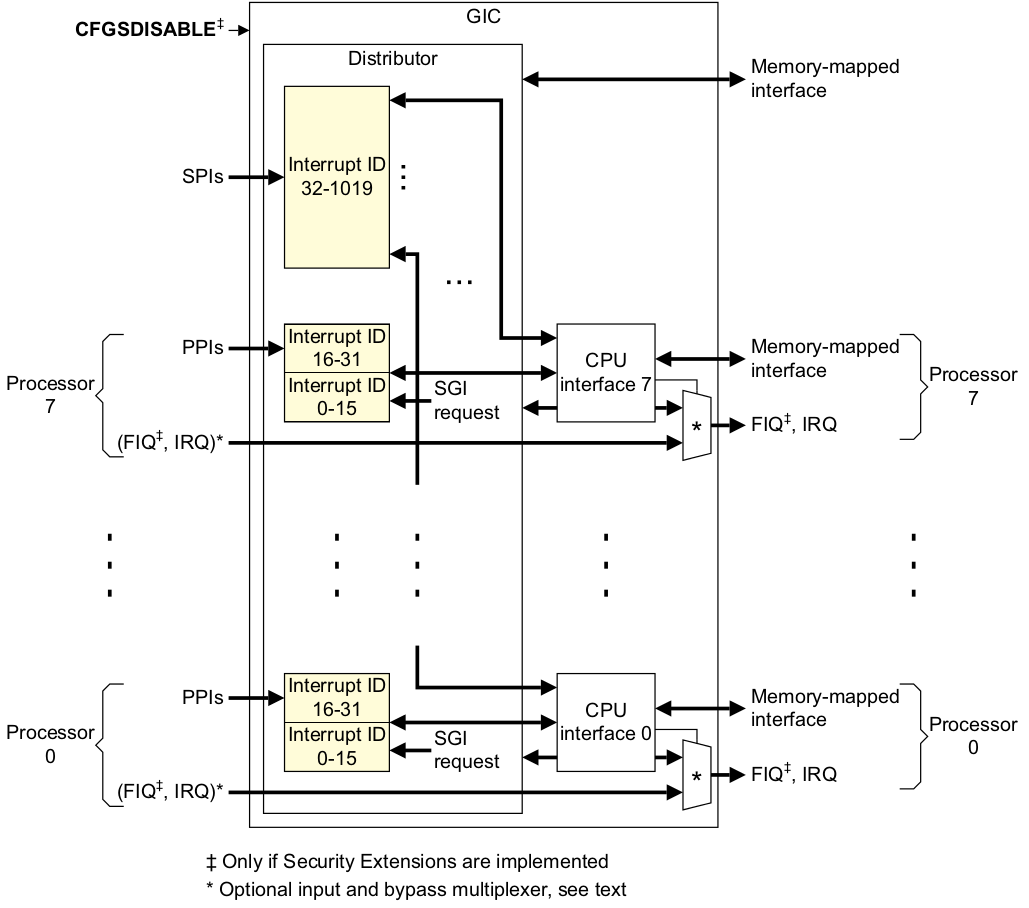
\includegraphics[width=9.5cm]{figuras/gic}
    \caption{Divisão lógica do GIC.}
    \label{img:gic}
\end{figure}

\subsection{Inicialização}

Na inicialização do distribuidor, através dos registradores mapeados em memória de configuração do mesmo, é definido, para cada uma das possíveis interrupções, se elas são \emph{level-sensitive} ou \emph{edge-triggered}.
Em seguida configura-se a prioridade de cada interrupção. A princípio todas as interrupções foram definidas como tendo a mesma prioridade, mas isto é configurável caso necessário.
É configurado então o processador-alvo de cada interrupção, isto é, para quais interfaces de processador uma determinada interrupção será encaminhada. Finalmente então são ativadas as interrupções \cite{gic}.

A inicialização da interface do processador é mais simples. Primeiro se configura a máscara de prioridade da CPU, isto é, qual é o nível de prioridade mínimo que uma interrupção precisa ter para interromper aquele processador. Na implementação, esta máscara está desativada. Depois configura-se a política de grupos de preempção. No GIC é possível separar interrupções em grupos de preempção, onde se define se determinado grupo pode preemptar determinado outro grupo. Todas as interrupções foram colocadas no mesmo grupo e interrupções podem ser preemptadas.

Adicionalmente a estas configurações, é possível de mascarar as interrupções FIQ e IRQ através do CPSR (\emph{Current Program Status Register}), alterando-se os bits 6 e 7 dele, para mascarar interrupções FIQ e IRQ, respectivamente. Normalmente é o que é feito quando é necessário mascaras as interrupções, enquanto se mantém as configurações do GIC.

\subsection{Fluxo de execução ao se receber uma interrupção}

O processador, ao receber uma interrupção, (portanto as interrupções estão ativas e não mascaradas pela interface ou pelo CPSR), para a execução do código que estava executando e então executa a instrução contida na tabela de vetores (mostrada na página \pageref{dump}) correspondente ao tipo de interrupção recebida. Esta instrução é um \emph{jump} para um tratador (\emph{handler}) daquele tipo de interrupção.

O principal tratador é o tratador de interrupções IRQ (\verb+irc_handler+), sendo que este precisa ser discutido com mais profundidade. Abaixo segue o código deste tratador:

\begin{verbatim}
 43 void _irq_handler() {
 44   ASMV(
 45   // A few definitions
 46   ".equ ARM_MODE_FIQ,      0x11 \n"
 47   ".equ ARM_MODE_IRQ,      0x12 \n"
 48   ".equ ARM_MODE_SVC,      0x13 \n"
 49   ".equ IRQ_BIT,           0x80 \n"
 50   ".equ FIQ_BIT,           0x40 \n"
 51 
 52   "msr cpsr_c, #ARM_MODE_SVC | IRQ_BIT | FIQ_BIT \n" // go to SVC
 53   // save current context (lr, sp and spsr are banked registers)
 54   "stmfd sp!, {r0-r3,r12,lr,pc}\n"
 55 
 56   "msr cpsr_c, #ARM_MODE_IRQ | IRQ_BIT | FIQ_BIT\n" //go to IRQ
 57 
 58   "sub r0, lr, #4 \n" // return from irq addr
 59   "mrs r1, spsr   \n" // pass irq_spsr to svc r1
 60 
 61   "msr cpsr_c, #ARM_MODE_SVC | IRQ_BIT | FIQ_BIT\n"//go back to SVC
 62   "add r2, sp, #24 \n"  // sp+24 is the position of the saved pc
 63   
 64   // save return address into the pc position
 65   "str r0, [r2] \n" 
 66   "stmfd sp!, {r1} \n"   // save irq-spsr
 67       
 68   );    
 69   
 70     
 71   IC::int_handler();
 72     
 73   ASMV(        
 74   "ldmfd sp!, {r0}              \n"
 75   "msr spsr_cfxs, r0\n"//restore IRQ's spsr value
 76                        //to SVC's spsr             
 77   "ldmfd sp!, {r0-r3,r12,lr,pc}^ \n" // restore context
 78   //the ^ in the end of the above instruction makes the 
 79   //spsr to be restored into svc_cpsr
 80   );
 81 }
\end{verbatim}

Após selecionar qual handler chamar, o processador muda de modo, indo, no caso de uma interrupção IRQ, para o modo de execução IRQ. Neste modo há 3 registradores banqueados: O SPSR, que contém o valor do registrador CPSR imediatamente antes da interrupção, sendo necessário para que seja possível restaurar o valor original do CPSR após tratar a interupção; o LR (\emph{link register}), que contém o endereço da próxima instrução que seria executada imediatamente antes da interrupção mais 4; e, finalmente, o SP (\emph{stack pointer}), que aponta para a pilha própria desde modo (cada modo pode possuir sua própria pilha).

Para evitar desperdício de memória reservando uma pilha própria apenas para este modo, optou-se por não usar uma pilha no modo IRQ, e, no lugar disto, usar sempre a mesma pilha do modo supervisor (que é o modo de execução do processador quando ele inicia). Para isto, a primeira instrução a executar é uma mudança de modo para voltar ao modo supervisor, enquanto mantendo novas interrupções desligadas; lá é salvo o contexto na pilha daquele modo. Entretanto para que seja possível restaurar o fluxo de execução no mesmo estado em que o processador estava no momento imediatamente antes da interrupção, é necessário voltar ao modo IRQ para obter-se os valores contidos dos registradores banqueados SPSR e LR; após isto, pode-se então voltar ao modo \emph{supervisor}. Na linha 62 do código é somado 24 à pilha pois lá é a posição de memória onde está salvo o PC após ele ter sido empilhado na linha 54, e deseja-se sobreescrever aquele valor do PC pelo valor que estava contido no LR do modo IRQ (menos 4), pois aquela é a próxima instrução que seria executada antes da interrupção. Feito isto, salva-se o valor do SPSR do modo IRQ no topo da pilha (que é o valor do CPSR pré-interrupção), para ser restaurado ao CPSR mais tarde.

Agora que o contexto foi salvo corretamente para ser restaurado, pode-se então chamar um tratador de interrupções genérico (que será discutido mais a frente) e escrito em C++. Após o \verb+int_handler+ da linha 71 retornar, é feita a restauração do contexto. Primeiro se salva o CPSR salvo na pilha no SPSR, na última instrução (\verb+ldmfd+), na forma em que ela está (com um \^{} no final dela e com o PC na lista), ela automaticamente restaurará o valor que está no SPSR para o CPSR. Como o PC está na lista, o fluxo de execução terá retornado a executar as instruções de antes da interrupção ocorrer.

Agora será discutido como que as interrupções são tratadas individualmente. O corpo do \verb+int_handler+ é bastante curto, então vale a pena escreve-lo aqui:

\begin{verbatim}
void Zynq_IC::int_handler()
{	
    unsigned int icciar_value = CPU::in32(IC::GIC_PROC_INTERFACE 
        | IC::ICCIAR);
    IC::Interrupt_Id id = icciar_value & IC::INTERRUPT_MASK;

    if(id == 1023){
        kout << "Spurious interruption received\n";
        return;
    }
    _vector[id](id);
    CPU::out32(IC::GIC_PROC_INTERFACE | IC::ICCEOI, icciar_value);
}
\end{verbatim}

A primeira coisa que o tratador faz e descobrir qual é o número da interrupção que foi gerada, para assim saber como tratar aquela interrupção. Isto é feito lendo-se o registrador ICCIAR (\emph{Interrupt Acknowledge Register}), que provê o número da interrupção e também o processador endereçado.
É possível que uma interrupção já tenha sido tratada por outro processador, quando isto acontece, o GIC emite uma \emph{Spurious Interruption} para indicar isto. Quando se detecta isto, o tratador não precisa tomar nenhuma outra ação, basta retornar a execução normal.

Com o número da interrupção em mãos, pode-se então chamar o tratador daquele tipo de interrupção. O \verb+_vector+ é um vetor de \emph{handlers}, onde para cada posição $i$, existe o tratador da interrupção número $i$. Para sinalizar que uma interrupção foi tratada, deve-se escrever no registrador ICCEOI (\emph{End of Interruption}) o número lido no ICCIAR (ou seja, o número da interrupção e processador de destino).


Normalmente, interrupções de \emph{timer} são o tipo mais frequente de interrupção durante a execução do sistema. Dele dependem o escalonador de processos (ou \emph{threads}), Delay, Chronometer e Alarm. Como mencionado na seção do porte do \emph{timer}, uma mesma interrupção pode gerar a chamada de mais de um handler, como a do \emph{timer} que chama a do Alarm e do escalonador. Com isto fica ilustrado que uma única interrupção pode gerar a chamada de vários tratadores para esta mesma interrupção.




\section{MMU}

%nice image in p.87 ug585

%na inicialização, é liberada toda a memória, colocando ela numa lista
%MMU é inteiramente controlada pelo coprocessador CP15
%http://www.slideshare.net/prabindh/enabling-two-level-translation-tables-in-armv7-mmu
%http://www.embedded-bits.co.uk/2011/mmucode/
%http://lxr.free-electrons.com/source/arch/arm/mm/proc-v7-2level.S?a=arm


%primeiro explica o motivo de existência da tabela né. diz que ela fica em alguma posição predeterminada da memória e que deve ser populada
%depois de dizer que ela deve ser populada, deve-se explicar o formato em baixo níve de cada página, para explicar com o que se está populando aquela tabela. depois disso a mmu traduz automagicamente.
%Como popular? não vou fazer 1-1 =p

%a mmu é toda controlada pelo coprocessador cp15, assim como lá existe alguns registradores que guardam informaçõos como o registrador que quarda o endereço base da TTB (translation table base) TTBR0 é o registrador da TT L1. (ARM ARM 1387). TTBR1 é para o SO e não muda durante troca de contexto.
%proteção de memória é feita pois pode-se mexer nos bits de dominio e tal, e cada thread possui um contexto e uma tabela mmu diferente, wtf.

%formato da l1 e l2 entries arm arm p.1282.


As principais funções de uma MMU (\emph{Memory Managemend Unit}) são proteção de memória, ou seja, de não permitir acesso a certas regiões da memória por processos/threads não autorizados, e de fazer o mapeamento de memória virtual para memória física, mapeamento este que facilita a escrita de aplicações já que o desenvolvedor dela não precisará estar ciente de como a memória é mapeada internamente pelo sistema operacional.

A MMU consegue cumprir estes dois objetivos (e outros mais) através do uso de uma tabela de tradução de página (que chamaremos de TTP), onde, a grosso modo, cada linha desta tabela é indexada pelo valor do endereço virtual, e na entrada correspondente há o endereço físico assim como \emph{flags} que indicam, dentre outras coisas, se aquela região pode ou não ser acessada pela aplicação corrente.

Esta tabela é salva na memória principal (RAM) do sistema, e configurar a MMU significa especialmente criar métodos para gerenciar e popular esta tabela. Para entender como isto é feito, será explicado agora como é estruturada esta tabela, como que ocorre a tradução de memória virtual para física, e o que cada entrada da tabela deve ter.

\subsection{Estrutura da Tabela de Tradução de Página}

Há, na realidade, mais que somente uma TTP. A TTP possui dois níveis, portanto, desconsiderando-se a TLB, é necessário dois acessos à TTB para se traduzir um endereço, caso configurado para páginas de 4 KB. a MMU suporta páginas de 4 KB e 64 KB, assim como seções de 1 MB e 16 MB. Como cada endereço virtual corresponde à exatamente uma entrada na TTP, usar páginas grandes reduz o tamanho da TTP (consequentemente o uso de memória por ela), entretanto usar páginas menores (4 KB) melhoram muito a eficiência da alocação dinâmica de memória e desfragmentação \cite[p.~77]{ug585.1.7}, porém mapear um espaço de 4 GB exigiria milhões de entradas na tabela. Foi justamente para conciliar estes fatores, que decidiu-se por uma tabela de dois níveis, como será melhor ilustrado a seguir.

A tabela de tradução páginas nível um (TTP1), também chamada de ``\emph{master table}'', divide todo o espaço de endereçamento de 4 GB em 4096 seções de 1 MB, portanto, como cada entrada desta tabela tem o tamanho de uma palavra, seu tamanho total em memória é de $4 \times 4096 = 16$ KB. Os 2 bits menos significativos (lsb) de cada entrada desta tabela, definem que tipo de entrada ela é, que pode ser um dos 4 tipos:

\begin{itemize}
	\item Bits 00: É uma ``fault entry'', e gera uma exceção do tipo \emph{prefetch} ou \emph{data abort}, dependendo do tipo de acesso. Este tipo de entrada indica que não há mapeamento virtual para esta região.
	\item Bits lsb 01: Indica a posição de memória para uma tabela de páginas (nível 2).
	\item Bits lsb 10 com bit 18 em 0: Aponta para uma seção de 1 MB.
	\item Bits lsb 10 com bit 18 em 1: Indica uma seção de 16 MB, este tipo de entrada exige 16 posições na TTB1.
	\item Bits lsb 11: Reservado, gera faltas de tradução e não deve ser usado.
\end{itemize}

A figura \ref{img:l1_entry} ilustra o formato de uma entrada da TTP1. NS significa \emph{non-secure}, e só tem semantica com extenções de segurança habilitadas (fora do escopo do trabalho). SBZ significa \emph{should be zero}. Bits C, B, TEX e AP serão explicados após a explicação do formato de uma entrada da TTP2, pois esta tem campos análogos.

\begin{figure}[hb!]
    \centering
    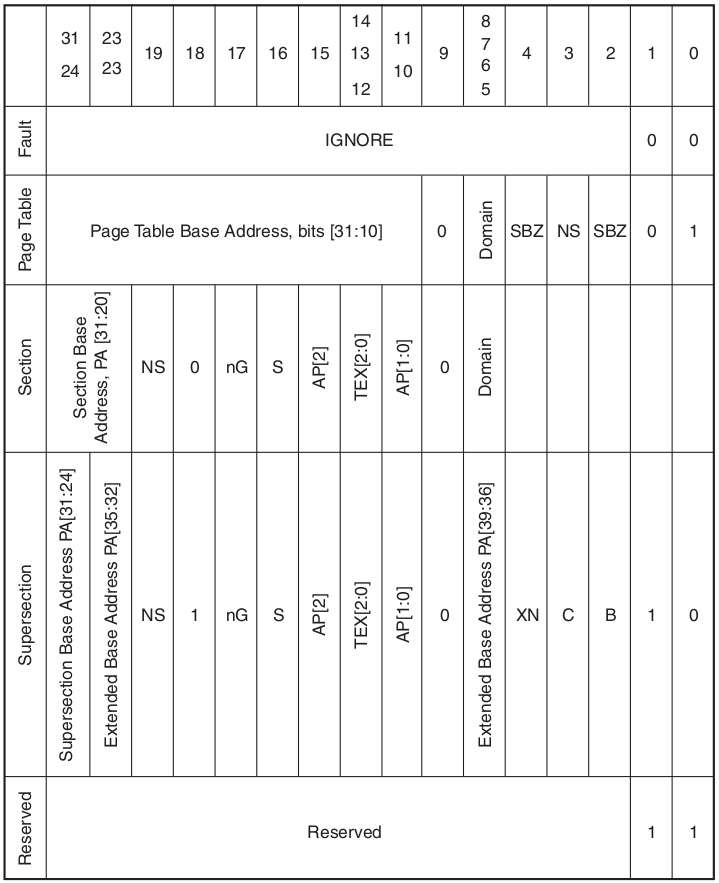
\includegraphics[width=9cm]{figuras/l1_entry}
    \caption{Divisão lógica do GIC.}
    \label{img:l1_entry}
\end{figure}

Vamos agora entender como se traduz de um endereço virtual, para uma TTP2. No coprocessador CP15, existe um registrador chamado TTBR (dois na realidade, TTBR0 e TTBR1), sigla de \emph{Translate Table Base Register}, onde é guardado o endereço da primeira posição da TTP1. Com a MMU ligada, quando há um acesso à memória, automaticamente a MMU pulará para a posição indicada no TTBR, e indexará esta tabela usando os 12 bits mais significativos do endereço virtual. A maneira exata de como é feito este cálculo é mostrada na figura \ref{fig:translation}.

Na posição de memória encontrada no passo anterior, estará uma entrada da TTP1 no formato indicado na figura \ref{fig:l1_entry}. No caso de uma entrada que indica uma outra TTP, os primeiros 22 bits indicam o endereço onde estará esta tabela, com os demais bits em 0, com exceção do último e os do campo de domínio (que será explicado a seguir). Com estas informações, a MMU já pode localizar a posição da TTP2. Para saber qual das entradas da TTP2 deve ser selecionada, é usado os bits [19:12] do endereço virtual para indexar a TTP2.

Os 4 bits do campo de domínio indicam em qual dos possíveis 16 domínios de memória aquela região se encontra, um domínio é apenas um conjunto de regiões de memória. A utilidade disto é que se pode, para cada domínio, especificar como será o controle de acesso nele. Cada domínio pode estar configurado (pelo registrador DACR) como um dos três tipos de acesso: \emph{Acesso não permitido}, qualquer acesso a esta região gera uma falta de domínio; \emph{Cliente}, permissões de acesso são verificadas, e podem gerar uma falta de permissão caso; e \emph{Administradores}, onde permissões de acesso não são verificadas.

\begin{figure}[h]
    \centering
    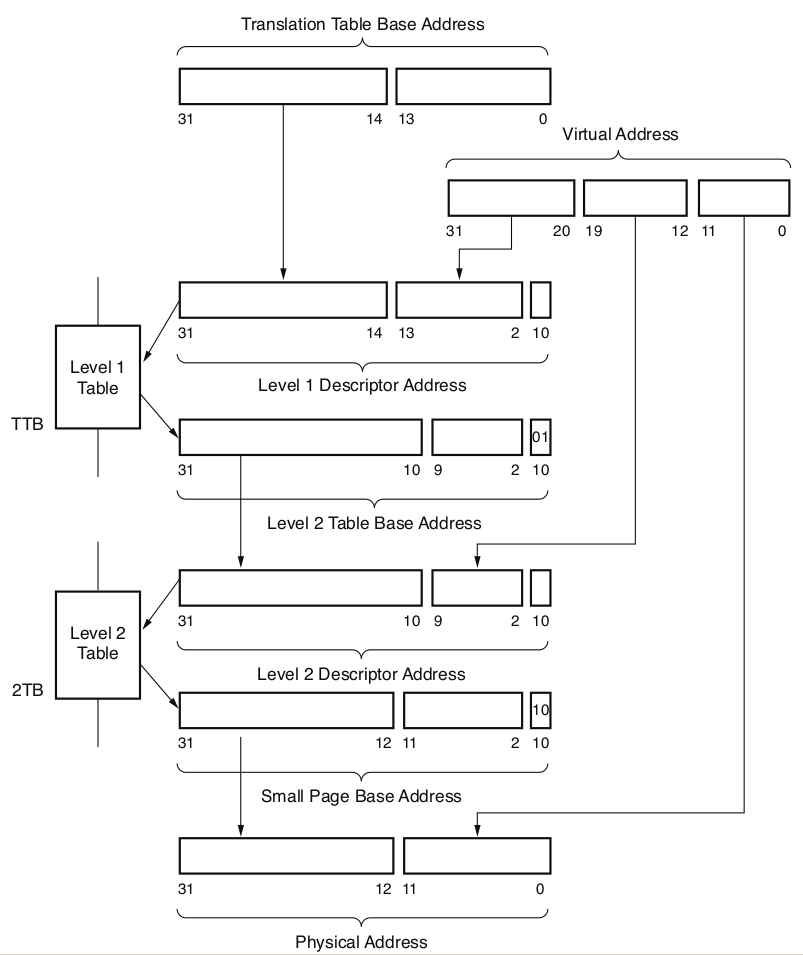
\includegraphics[width=9cm]{figuras/translation}
    \caption{Divisão lógica do GIC.}
    \label{img:translation}
\end{figure}

A TTP2 possui 256 entradas, cada uma com o tamanho de uma palavra, logo, cada TTP2 precisa de 1 KB de memória. Note que como uma entrada da TTB1 provê 22 bits para endereçar uma TTP2, esta TTP2 pode efetivamente estar localizada em qualquer região da memória, já que 22 bits são suficientes para indexar qualquer região de 1 KB de memória.

A figura \ref{fig:l2_entry} ilustra como é o formato de uma entrada na TTP2. Os 2 bits menos significativos indicam se a página possui 4 KB, 16 KB ou se a região não está mapeada. Com o endereço de uma entrada da TTP2 em mãos, basta combinar os 20 bits mais significativos desta entrada com os 12 bits menos significativos do endereço virtual, e teremos traduzido o endereço virtual para um físico.

\begin{figure}[h]
    \centering
    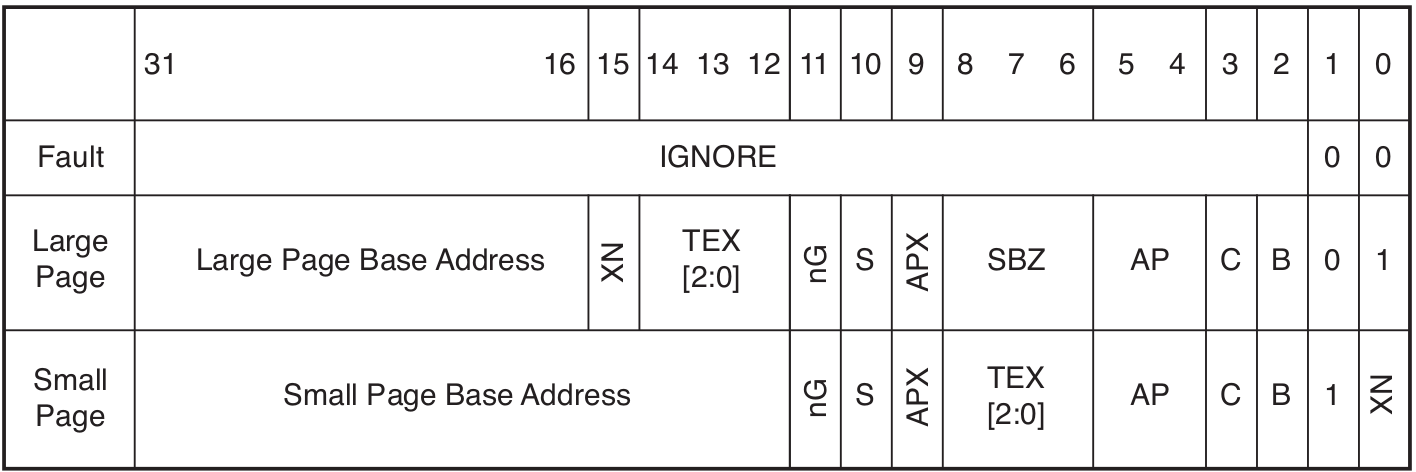
\includegraphics[width=9cm]{figuras/l2_entry}
    \caption{Divisão lógica do GIC.}
    \label{img:l2_entry}
\end{figure}

Agora vamos discutir o que cada campo de uma entrada da TTP2 significa.

\textbf{AP e APx:} São os bits que codificam o tipo de acesso que aquela porção de memória possui. Estes bits só são checados caso do domínio seja de \emph{Cliente}. Um acesso que não possui as permissões necessárias geram uma exceção do tipo \emph{prefetch} ou \emph{data abort}. APx e AP[2] são sinônimos. A tabela \ref{tab:apx} ilustra os diferentes tipos de acesso que podem ser codificados.

\begin{table}[h]
	\centering
	\begin{tabular}{cccccc}
		\hline \hline
		APx & AP[1] & AP[0] & Acesso privilegiado & Acesso não privilegiado & Descrição\\[0.5ex]
		\hline
		0 & 0 & 0 & Sem acesso & Sem acesso & Gera uma falta de permissão\\
		0 & 0 & 1 & Escrita/Leitura & Sem acesso & Acesso somente modo privilegiado\\
		0 & 1 & 0 & Escrita/Leitura & Sem acesso & Acesso somente modo privilegiado\\
		0 & 1 & 1 & Escrita/Leitura & Sem acesso & Acesso somente modo privilegiado\\
		1 & 0 & 0 & \~{} 			& \~{}		 & Combinação reservada\\
		1 & 0 & 1 & Leitura 		& Sem acesso & Leitura somente modo privilegiado\\
		1 & 1 & 0 & Leitura 		& Leitura	 & Somente leitura\\
		1 & 1 & 1 & \~{} 			& \~{}		 & Combinação reservada\\[1ex]
		\hline
	\end{tabular}
	\caption{Codificações das permissões de acesso.}
	\label{tab:apx}
\end{table}

\textbf{TEX:} Controla políticas de compartilhamento de memória, caso aquela região seja compartilhada.
\textbf{C e B:} Estes campos combinados controlam a política de ``cacheamento'' daquela região de memória, ou seja, se ela pode ser salva na cache, e se pode, qual o algoritmo a a ser usado, como \emph{write-back} ou \emph{write-though}, e também políticas de \emph{write-allocate}.
\textbf{S:} Bit que determina que aquela porção de memória é compartilhada entre processadores.
\textbf{nG:} Responsável pela proteção de memória intraprocessos. Uma região marcada como não global (nG = 1) tem associado à ela um número que o SO atribui a cada processo. Isto permite que a TLP possa ter diferentes mapeamentos simultaneamente sem necessidade de substituir uma entrada.
\textbf{xN:} Bit que marca a região como não executável. É importante por questões de segurança, já que o \emph{fetch} especulativo de instruções pode ler uma porção de memória que possui dados sensíveis.


\subsection{Populando a Tabela}

Agora que sabemos como as TTPs são estruturadas, bem como o formato de cada entrada dela, podemos finalmente popular esta tabela. Há várias estratégias para fazer isto \cite{mmutheory}, dependendo da forma desejada de mapeamento, por exemplo:

\begin{itemize}
	\item Mapeamento por Demanda: Pode-se fazer com que determinado endereço virtual não possua um mapeamento correspondente a priori, gerando uma exceção que é tratada criando-se uma TTP2 que mapeie aquela área.
	\item Mapeamento 1 para N: Com o advento do bit nG, é possível também mapear uma mesma área de memória virtual em diferentes áreas da memória física, de modo que quando o escalonador de processos escalona num novo processo (ou \emph{thread}), ele também modifica o mapeamento de memória, deste modo, diferentes processos poderiam usar uma mesma determinada posição de memória virtual.
	\item Mapeamento 1 para 1: É o mapeamento mais simples possível, de modo que a posição de memória virtual X corresponde a posição de memória física X; foi usado este mapeamento para validação de permissões.
\end{itemize}

Em um mapeamento 1 para 1, para popular as TTBs, primeiramente, em um loop, itera-se 512 vezes (já que há 512 de RAM), salvando em posições sucessivas de uma determinada região da memória os endereços das TTB2s, levando-se em conta as \emph{flags} acima mencionadas, após as 512 posições, itera-se pelas 3584 posições restantes (4 GB - 512 MB) marcando aquelas regiões como não mapeadas. Feito isto, é necessário também popular cada TTB2 que foi apontada na TTB1, em um processo semelhante. Em um mapeamento por demanda, marca-se as regiões da memória virtual como não mapeadas, com a diferença que, ao invés de apenas abortar o acesso, cria-se dinamicamente aquele mapeamento.

Após feita as tabelas, a MMU está pronta para ser ativada. A MMU é controlada pelo coprocessador CP15, é nele que são guardados os registradores de configuração, endereço base para a TTP, dentre outras funções. Escrevendo-se 1 no bit menos significativo no registrador c1 (SCTLR) deste coprocessador a MMU é ativada.

%memory map?

\section{Multicore}

%Ativar o segundo processador exige poucas linhas de código
Ao se ligar a placa, apenas a CPU0 executa código, e é função dela fazer as inicializações necessárias para então ligar o segundo processador (CPU1). Inicialmente, o CPU1 executa uma instrução (\verb+wfe+) que o coloca em modo de espera por evento (\emph{Wait for Event Mode}). Para sair deste modo, a CPU0 precisa emitir uma instrução do tipo evento de sistema, \verb+sev+ (\emph{System Event}). Quando a CPU1 recebe este sinal, ele imediatamente executa a instrução que está no endereço 0xfffffff0, localização onde a CPU0 deve previamente ter escrito uma instrução que faça a CPU1 fazer um \verb+jump+ para o ponto de entrada do que se deseja executar com a CPU1. Note que a posição 0xfffffff0 é uma região reservada da memória, e não corresponde à uma posição da RAM (é o mesmo princípio de registradores mapeados em memória).

Isto é suficiente para fazer o segundo processador passar a executar código, entretanto esta é a parte simples, ter dois processadores rodando tem várias implicações sobre como deve ser o \emph{design} de cada componente do sistema, pois agora há a preocupação com coerência e consistência de memória, condições de corrida {\emph{racing conditions}) e etc.

\chapter{Conclusão}

Este trabalho visou descrever como foi feito o porte do sistema operacional EPOS para a Zedboard. Foram explicadas as decisões de projeto feitas, de modo que as próximas pessoas que venham a portar o EPOS para outra arquitetura, possam entender o raciocínio por trás do que foi implementado, de modo que o que foi aqui exposto possa ser adaptado para outros contextos.

Foi necessário explicar uma série de especificidades da arquitetura para expor como que é feito o interfaceamento do software com o hardware, e como um sistema operacional pode controlar e configurar componentes de hardware.

Este porte possibilitou novos cenários de aplicação do EPOS, espera-se portanto que isto contribua para estimular novas linhas de pesquisa com este sistema operacional.
